%Este trabalho está licenciado sob a Licença Atribuição-CompartilhaIgual 4.0 Internacional Creative Commons. Para visualizar uma cópia desta licença, visite http://creativecommons.org/licenses/by-sa/4.0/deed.pt_BR ou mande uma carta para Creative Commons, PO Box 1866, Mountain View, CA 94042, USA.

\chapter{Interpolação}\label{cap_interp}
\thispagestyle{fancy}

Neste capítulo, discutiremos sobre a resolução de problemas de interpolação da forma: dados uma família de $n$ funções reais $\mathcal{F} = \{f_1(x), f_2(x), \ldots, f_n(x)\}$ e um conjunto de $n$ pontos $\{(x_i, y_i)\}_{i=1}^n$, com $x_i\neq x_j$ se $i\neq j$, encontrar
\begin{equation}
  f(x) = c_1f_1(x) + c_2f_2(x) + \cdots + c_nf_n(x),
\end{equation}
tal que
\begin{equation}
  y_i = f(x_i),\quad i=1, 2, \ldots, n.
\end{equation}

\section{Interpolação polinomial}\label{cap_interp_sec_interpoli}

Dado um conjunto de $n$ pontos $\{(x_i, y_i)\}_{i=1}^n$, o problema de interpolação consiste em encontrar o polinômio de grau $n-1$
\begin{equation}\label{eq:interpoli_poli}
  p(x) = p_1x^{n-1} + p_2x^{n-2} + \cdots + p_{n-1}x + p_n
\end{equation}
tal que
\begin{equation}\label{eq:interpoli_conds}
  y_i = p(x_i),\quad i=1, 2, \ldots, n.
\end{equation}

Das condições \eqref{eq:interpoli_poli}, temos
\begin{align}\label{eq:interpoli_sis}
  p_1x_1^{n-1} + p_2x_1^{n-2} + \cdots + p_{n-1}x_1 + p_n &= y_1 \\
  p_1x_2^{n-1} + p_2x_2^{n-2} + \cdots + p_{n-1}x_2 + p_n &= y_2 \\
  &\vdots \\
  p_1x_n^{n-1} + p_2x_n^{n-2} + \cdots + p_{n-1}x_n + p_n &= y_n.
\end{align}
Isto é, os coeficientes do polinômio interpolador \eqref{eq:interpoli_poli} satisfazem o seguinte sistema linear
\begin{equation}
  A\pmb{p} = \pmb{y},
\end{equation}
onde $A$ é a matriz de Vandermonde\footnote{Alexandre-Théophile Vandermonde, 1735 - 1796, matemático francês. Fonte: \href{https://en.wikipedia.org/wiki/Alexandre-Th\%C3\%A9ophile_Vandermonde}{Wikipedia}.}
\begin{equation}
  A =
  \begin{bmatrix}
    x_1^{n-1} & x_1^{n-2} & \ldots & x_1 & 1 \\
    x_2^{n-1} & x_2^{n-2} & \ldots & x_2 & 1 \\
    \vdots  & \vdots  & \vdots  & \vdots & \vdots \\
    x_n^{n-1} & x_n^{n-2} & \ldots & x_n & 1
  \end{bmatrix},
\end{equation}
$\pmb{p} = (p_1, p_2, \ldots, p_n)$ é o vetor das incógnitas e $\pmb{y} = (y_1, y_2, \ldots, y_n)$ é o vetor dos termos constantes.

\begin{ex}\label{ex:interpoli_intro}
  Consideremos o problema de encontrar o polinômio interpolador do conjunto de pontos $\{(-1,~-1), (0,~1), (1,~1/2)\}$. Como temos 3 pontos, o polinômio tem grau 2 e pode ser escrito na forma
  \begin{equation}
    p(x) = p_1x^2 + p_2x + p_3.
  \end{equation}
  Seguindo a abordagem acima, temos $\pmb{p}=(p_1, p_2, p_3)$, $\pmb{x} = (-1, 0, 1)$, $\pmb{y}=(-1, 1, 1/2)$ e
  \begin{equation}
    A =
    \begin{bmatrix}
      x_1^2 & x_1 & 1\\
      x_2^2 & x_2 & 1\\
      x_3^2 & x_3 & 1
    \end{bmatrix}.
  \end{equation}
  Então, resolvendo $A\pmb{p} = \pmb{y}$, obtemos o polinômio interpolador
  \begin{equation}
    p(x) = -1,25x^2 + 0,75x + 1.
  \end{equation}
A Figura \ref{fig:interpoli_intro} mostra os esboços do polinômio interpolador $p(x)$ e  dos pontos dados.

\begin{figure}[h!]
  \centering
  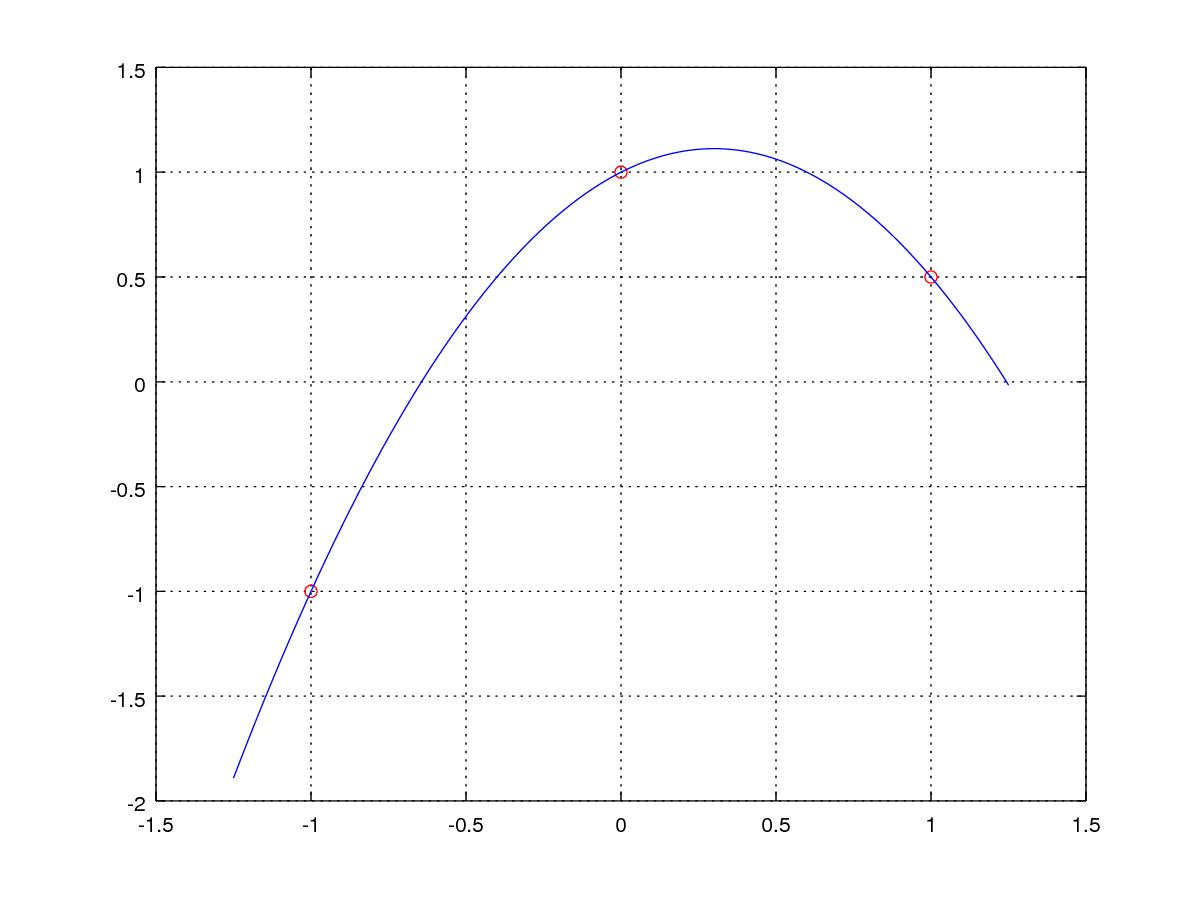
\includegraphics[width=0.7\textwidth]{./cap_interp/dados/ex_interpoli_intro/fig_interpoli_intro}
  \caption{Esboços dos pontos e do polinômio interpolador referente ao Exemplo \ref{ex:interpoli_intro}.}
  \label{fig:interpoli_intro}
\end{figure}

\ifisoctave
No \verb+GNU Octave+, podemos fazer as computações acima com o seguinte \href{https://github.com/phkonzen/notas/blob/master/src/MatematicaNumerica/cap_interp/dados/ex_interpoli_intro/ex_interpoli_intro.m}{código}:
\verbatiminput{./cap_interp/dados/ex_interpoli_intro/ex_interpoli_intro.m}
\fi
\end{ex}

\subsection*{Exercícios}

\begin{exer}\label{exer:interpoli_intro1}
  Obtenha o polinômio interpolador do conjunto de pontos $\{(-1,~-1), (0,~1), (1,~1/2), (2,~1)\}$.
\end{exer}
\begin{resp}
\ifisoctave
\href{https://github.com/phkonzen/notas/blob/master/src/MatematicaNumerica/cap_interp/dados/exer_interpoli_intro1/exer_interpoli_intro1.m}{Código}.
\fi
$0,58\bar{3}x^2 - 1,25x + 0,1\bar{6} + 1$.  
\end{resp}

\emconstrucao

\section{Interpolação de Lagrange}\label{cap_interp_sec_lagrange}

Interpolação de Lagrange\footnote{Joseph-Louis Lagrange, 1736 - 1813, matemático italiano. Fonte: \href{https://en.wikipedia.org/wiki/Joseph-Louis_Lagrange}{Wikipedia}.} é uma técnica para a computação do polinômio interpolador $p(x)$ de um conjunto de pontos $\{(x_i, y_i)\}_{i=1}^n$ dados. A ideia consiste em escrever o polinômio interpolador na forma
\begin{equation}
  p(x) = y_1L_1(x) + y_2L_2(x) + \cdots + y_nL_n(x),
\end{equation}
onde $L_i(x)$ é chamado de $i$-ésimo polinômio de Lagrange e é definido como o polinômio de grau $n-1$ que satisfaz
\begin{equation}
  L_i(x_j) = \left\{
    \begin{array}{ll}
      1 &, i=j\\
      0 &, i\neq j
    \end{array}
\right.
\end{equation}
Mais especificamente, temos que $L_i(x)$ tem raízes $\{x_1, \ldots, x_{i-1}, x_{i+1}, \ldots, x_n\}$ e, portanto, pode ser decomposto na forma
\begin{equation}
  L_i(x) = c_i(x-x_1)\cdots(x-x_{i-1})(x-x_i)\cdots(x-x_n).
\end{equation}
Além disso, como $L_i(x_i) = 1$, temos
\begin{equation}
  c_i = \frac{1}{(x_i-x_1)\cdots(x_i-x_{i-1})(x_i-x_i)\cdots(x_i-x_n)}.
\end{equation}
Assim sendo, podemos concluir que
\begin{equation}
  L_i(x) = \frac{(x-x_1)\cdots(x-x_{i-1})(x-x_i)\cdots(x-x_n)}{(x_i-x_1)\cdots(x_i-x_{i-1})(x_i-x_i)\cdots(x_i-x_n)}.
\end{equation}


\begin{ex}
  Consideremos o problema de encontrar o polinômio interpolador do conjunto de pontos $\{(-1,~-1), (0,~1), (1,~1/2)\}$. Como temos 3 pontos, o polinômio tem grau 2 e pode ser escrito na seguinte forma de Lagrange
  \begin{equation}
    p(x) = y_1L_1(x) + y_2L_2(x) + y_3L_3(x),
  \end{equation}
  onde $y_1 = -1$, $y_2 = 1$ e $y_3 = 1/2$. Os polinômios de Lagrange são dados por
  \begin{align}
    L_1(x) &= \frac{(x-x_2)(x-x_3)}{(x_1-x_2)(x_1-x_3)} = \frac{1}{2}x^2 - \frac{1}{2}x,\\
    L_2(x) &= \frac{(x-x_1)(x-x_3)}{(x_2-x_1)(x_2-x_3)} = -x^2 + 1,\\
    L_3(x) &= \frac{(x-x_1)(x-x_2)}{(x_3-x_1)(x_3-x_2)} = \frac{1}{2}x^2 + \frac{1}{2}x.\\
  \end{align}
  E, então, temos o polinômio interpolador
  \begin{equation}
    p(x) = -1,25x^2 + 0,75x + 1.
  \end{equation}

\ifisoctave
No \verb+GNU Octave+, podemos fazer as computações acima com o seguinte \href{https://github.com/phkonzen/notas/blob/master/src/MatematicaNumerica/cap_interp/dados/ex_interpoli_lagrange/ex_interpoli_lagrange.m}{código}:
\verbatiminput{./cap_interp/dados/ex_interpoli_lagrange/ex_interpoli_lagrange.m}
\fi
\end{ex}

\subsection{Aproximação de funções}

Polinômio interpoladores podem ser usados para a aproximação de funções. Podemos aproximar uma dada função $f$ pelo polinômio interpolador de um conjunto de pontos selecionados $\{(x_i, y_i=f(x_i))\}_{i=1}^n$. De fato, o seguinte teorema nos fornece uma estimativa para o erro de uma tal interpolação.

\begin{teo}(\normalfont{Teorema de Lagrange})\label{teo:lagrange}
  Sejam dados uma função $f$ $n+1$-vezes continuamente diferenciável em um dado intervalo $[a, b]$ e $n$ pontos $\{x_i\}_{i=1}^n\subset [a, b]$. Então, o polinômio interpolador do conjunto de pontos $\{x_i, y_i=f(x_i)\}_{i=1}^n$ satisfaz
  \begin{equation}
    f(x) = p(x) + \frac{f^{(n+1)}(\xi)}{(n+1)!}(x-x_1)(x-x_2)\cdots (x-x_n).
  \end{equation}
\end{teo}
\begin{dem}
  \emconstrucao
\end{dem}

\begin{ex}\label{ex:interpoli_aprox}
  Considere o problema de aproxima $f(x) = \sen(x)$ pelo polinômio interpolador pelo conjunto de pontos $x_1=0$, $x_2=\pi/2$ e $x_3=\pi$. Isto, queremos determinar o polinômio $p(x)$ de grau $2$ que interpola os pontos $\{(0,0),~(\pi/2,~1),~(\pi,0)\}$. Usando a técnica de Lagrange, obtemos
  \begin{equation}
    p(x) = -0,41x^2 + 1,3x,
  \end{equation}
com seus coeficientes arredondados para dois dígitos significativos. A Figura \ref{fig:interpoli_aprox} mostra os esboços da função $f(x)=\sen(x)$, dos pontos dados e do polinômio interpolador $p(x)$.

\begin{figure}[h!]
  \centering
  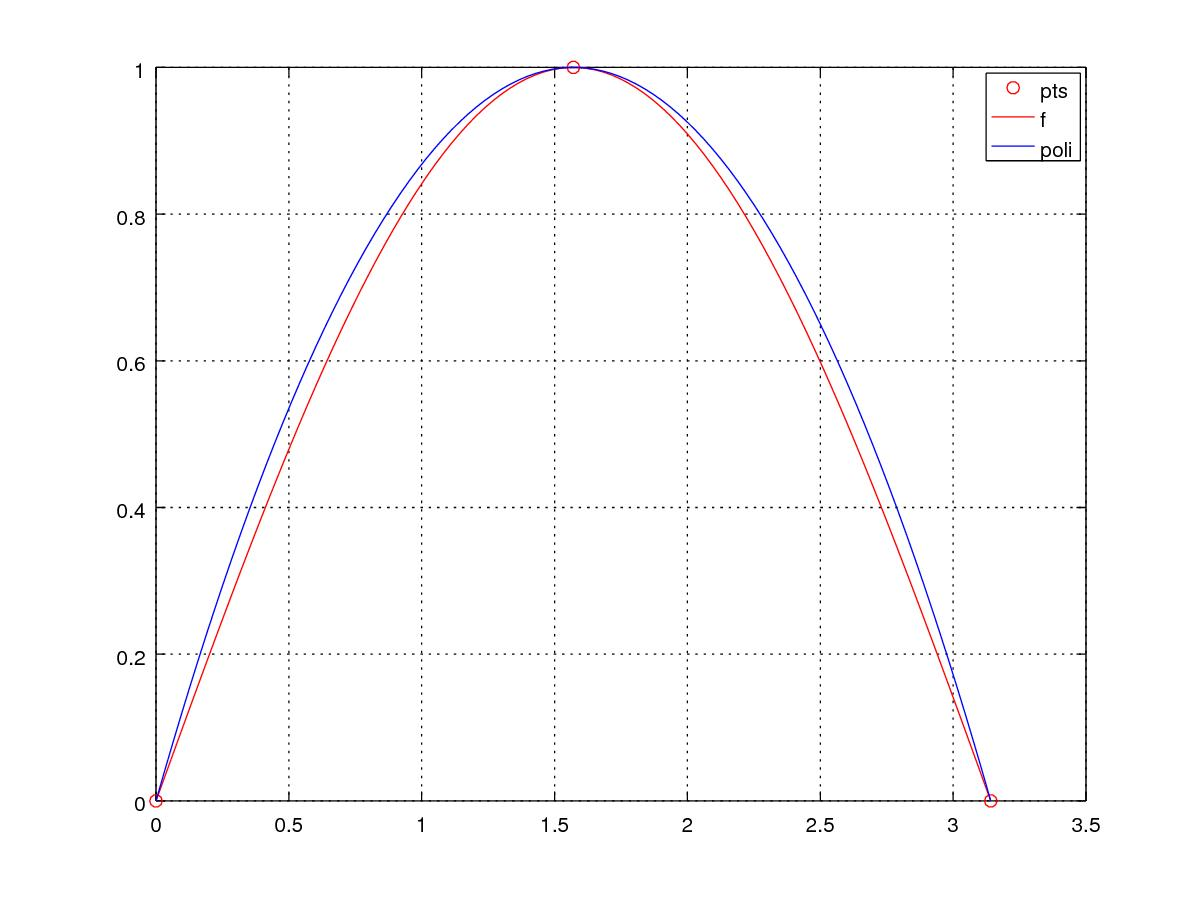
\includegraphics[width=0.7\textwidth]{./cap_interp/dados/ex_interpoli_aprox/fig_interpoli_aprox}
  \caption{Esboços dos gráficos da função, dos pontos e do polinômio interpolador computado no Exemplo \ref{ex:interpoli_aprox}.}
  \label{fig:interpoli_aprox}
\end{figure}

\ifisoctave
No \verb+GNU Octave+, podemos fazer as computações acima com o seguinte \href{https://github.com/phkonzen/notas/blob/master/src/MatematicaNumerica/cap_interp/dados/ex_interpoli_aprox/ex_interpoli_aprox.m}{código}:
\verbatiminput{./cap_interp/dados/ex_interpoli_aprox/ex_interpoli_aprox.m}
\fi
\end{ex}

\subsection*{Exercícios}

\begin{exer}
  Use a técnica de interpolação de Lagrange para encontrar o polinômio interpolador que aproxima a função$f(x)=e^{x}$ pelos pontos $x_1=0$, $x_2=1$, $x_3=1,5$ e $x_4=2$.
\end{exer}
\begin{resp}
\ifisoctave
\href{https://github.com/phkonzen/notas/blob/master/src/MatematicaNumerica/cap_interp/dados/exer_interpoli_aprox1/exer_interpoli_aprox1.m}{Código}.
\fi
$0,54x^3 - 0,15x^2 + 1,3x + 1$.
\end{resp}

\emconstrucao
